\documentclass[border=10pt, tikz]{standalone}
\usetikzlibrary{arrows.meta}

% Draw a single thin vertical slice
% #1=name, #2=x, #3=y, #4=height, #5=fill color
\newcommand{\slice}[5]{%
  \pgfmathsetmacro{\sw}{0.18}%  slice width
  \pgfmathsetmacro{\hh}{0.5*#4}%
  \filldraw[draw=blue!55!black, fill=#5, line width=0.5pt]
    (#2,#3-\hh) rectangle ++(\sw,#4);
  \coordinate (#1-west)  at (#2,#3);
  \coordinate (#1-east)  at (#2+\sw,#3);
  \coordinate (#1-north) at (#2+0.5*\sw,#3+\hh);
  \coordinate (#1-south) at (#2+0.5*\sw,#3-\hh);
}

\begin{document}
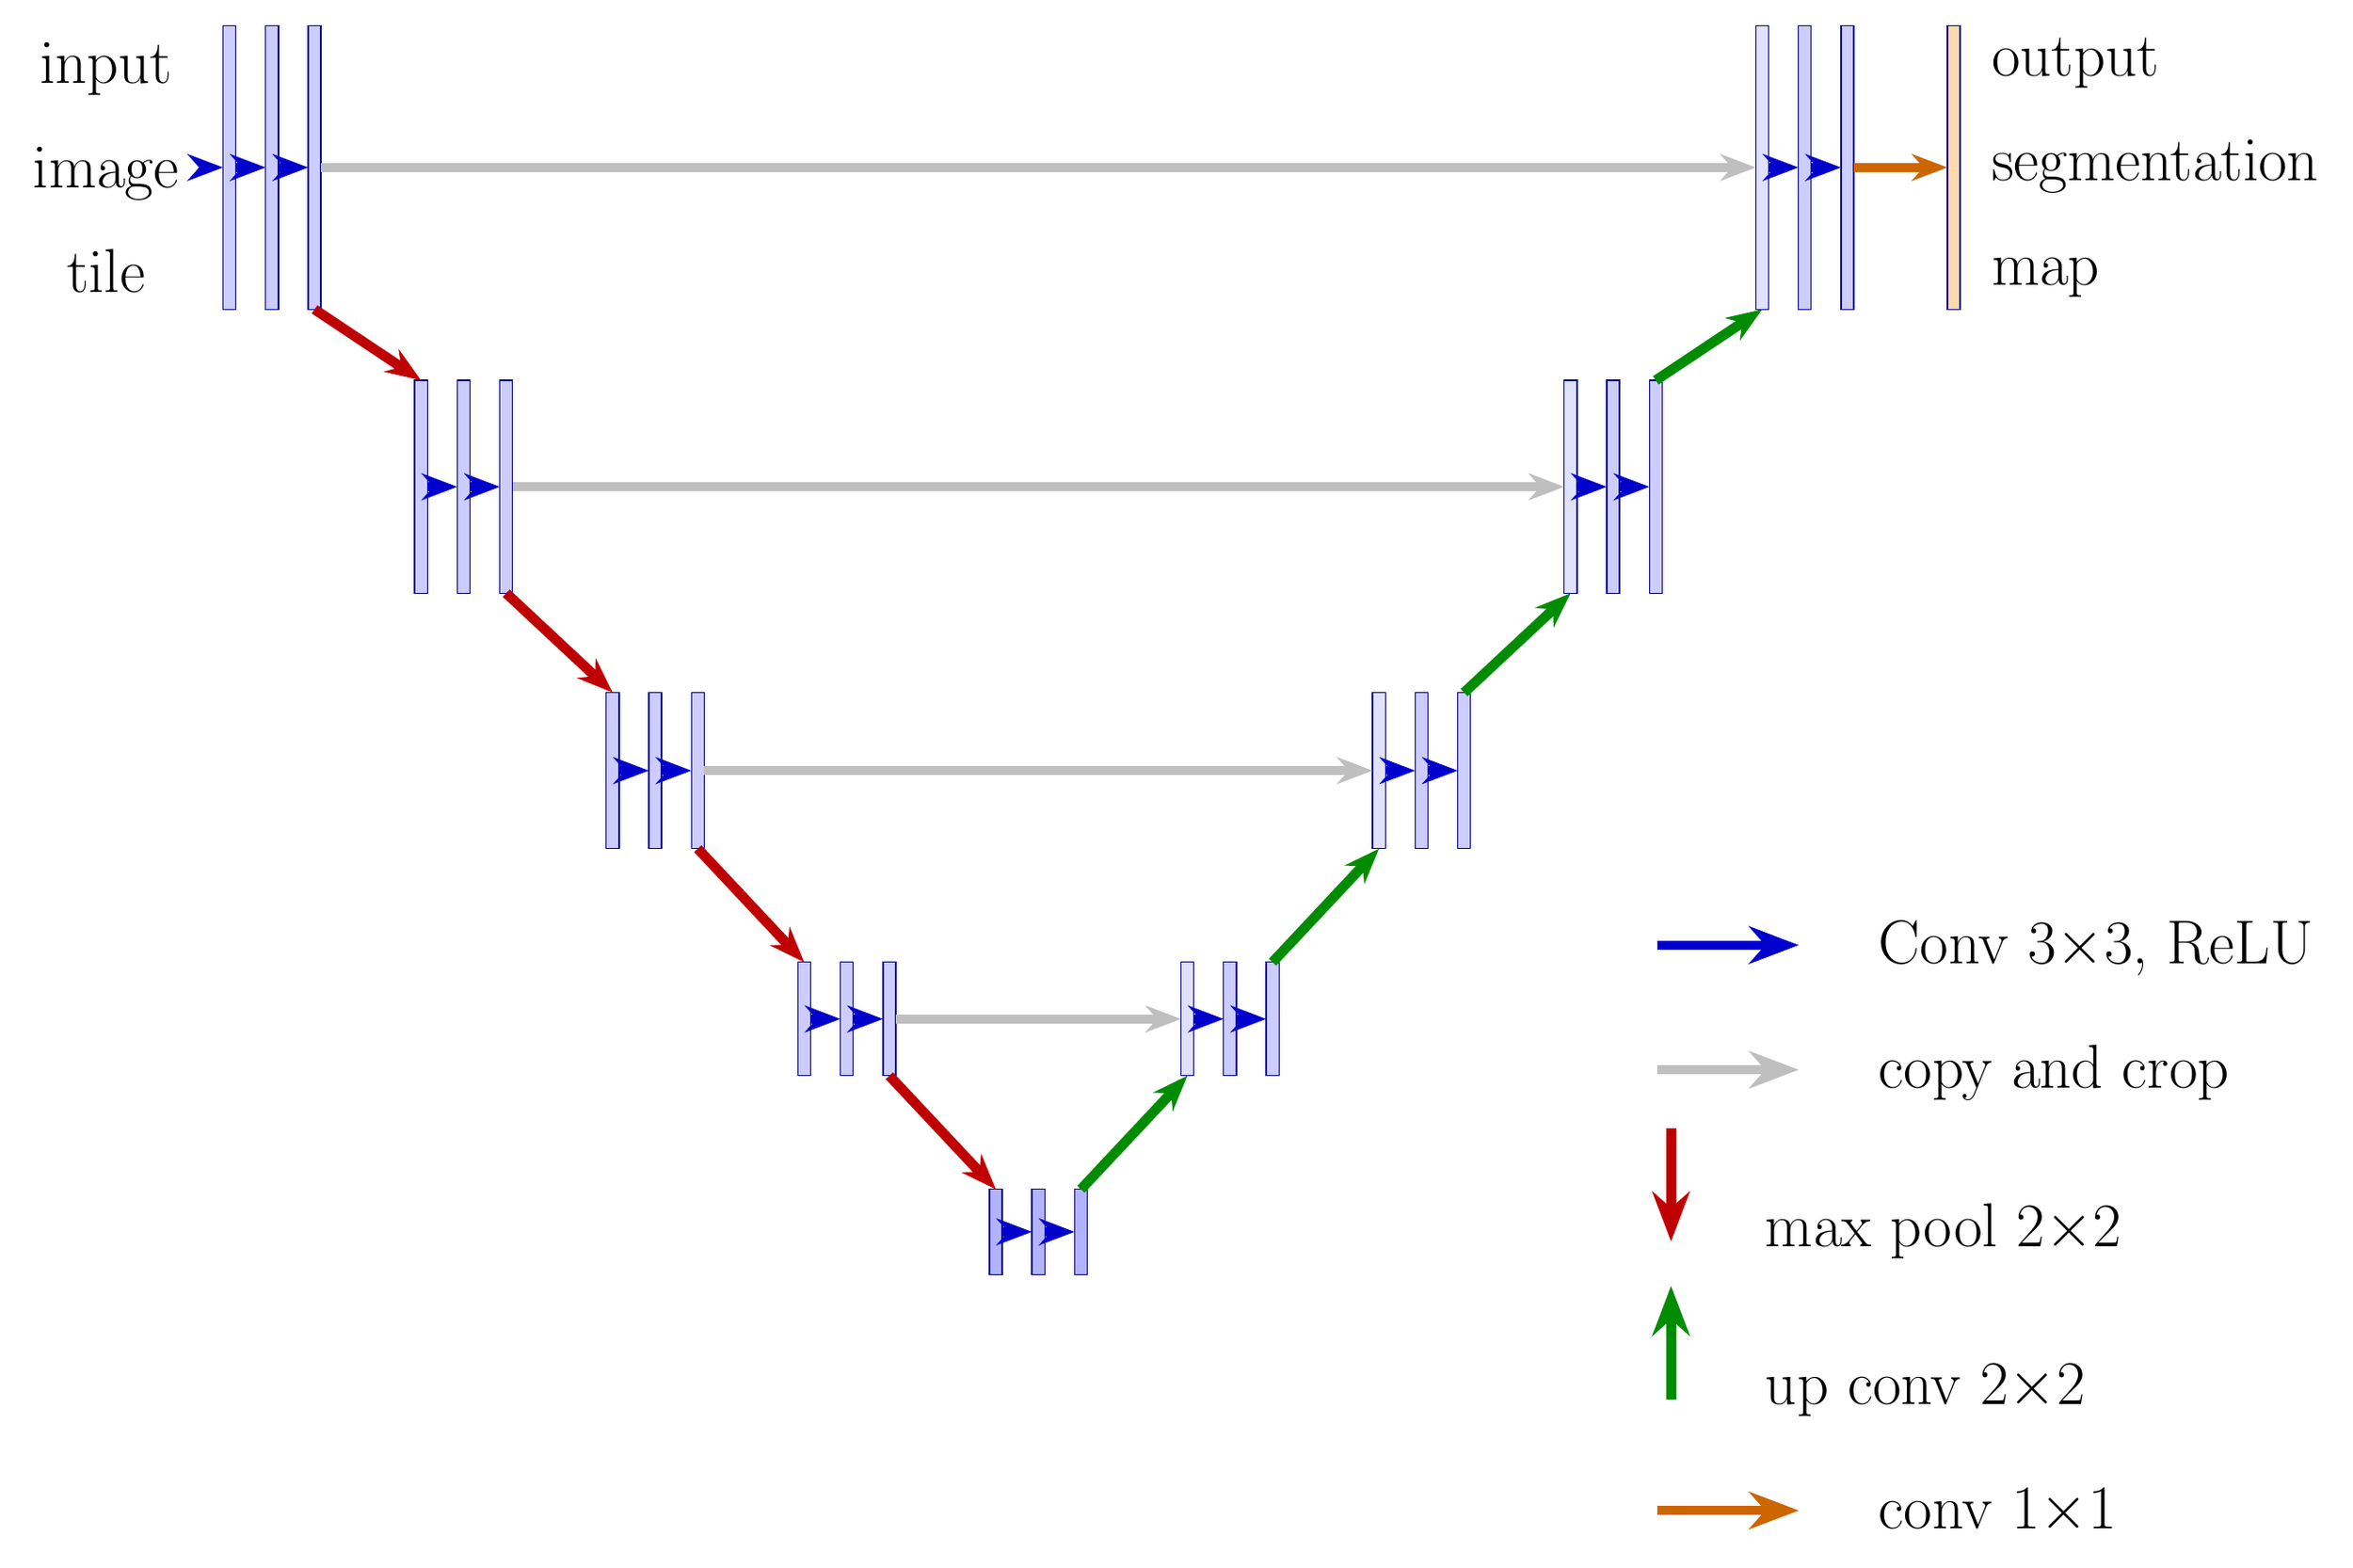
\begin{tikzpicture}[
  font=\fontsize{35}{42}\selectfont,
  conv/.style  = {-{Stealth[length=5.0mm]}, line width=3.6pt, draw=blue!80!black},
  skip/.style  = {-{Stealth[length=5.0mm]}, line width=3.6pt, draw=gray!50},
  pool/.style  = {-{Stealth[length=5.0mm]}, line width=4.0pt, draw=red!75!black},
  upc/.style   = {-{Stealth[length=5.0mm]}, line width=4.0pt, draw=green!55!black},
  outc/.style  = {-{Stealth[length=5.0mm]}, line width=3.6pt, draw=orange!80!black},
]

% U-SHAPE layout: each encoder stage has 3 individual slices with arrows between them
% Each stage steps RIGHT and DOWN, bottleneck at bottom-center, decoder steps RIGHT and UP.
%
% x: ~0.6cm between slices in a stage, ~1.5cm gap to next stage
% y: rows at 0, -4.5, -8.5, -12.0, -15.0
% heights: 4.0, 3.0, 2.2, 1.6, 1.2

% --- Encoder Stage 1: y=0.0, h=4.0 (3 slices) ---
\slice{e1s1}{ 0.0}{ 0.0}{4.0}{blue!20}
\slice{e1s2}{ 0.6}{ 0.0}{4.0}{blue!20}
\slice{e1s3}{ 1.2}{ 0.0}{4.0}{blue!20}

% --- Encoder Stage 2: y=-4.5, h=3.0 ---
\slice{e2s1}{ 2.7}{-4.5}{3.0}{blue!20}
\slice{e2s2}{ 3.3}{-4.5}{3.0}{blue!20}
\slice{e2s3}{ 3.9}{-4.5}{3.0}{blue!20}

% --- Encoder Stage 3: y=-8.5, h=2.2 ---
\slice{e3s1}{ 5.4}{-8.5}{2.2}{blue!20}
\slice{e3s2}{ 6.0}{-8.5}{2.2}{blue!20}
\slice{e3s3}{ 6.6}{-8.5}{2.2}{blue!20}

% --- Encoder Stage 4: y=-12.0, h=1.6 ---
\slice{e4s1}{ 8.1}{-12.0}{1.6}{blue!20}
\slice{e4s2}{ 8.7}{-12.0}{1.6}{blue!20}
\slice{e4s3}{ 9.3}{-12.0}{1.6}{blue!20}

% --- Bottleneck: y=-15.0, h=1.2 ---
\slice{bn1}{10.8}{-15.0}{1.2}{blue!30}
\slice{bn2}{11.4}{-15.0}{1.2}{blue!30}
\slice{bn3}{12.0}{-15.0}{1.2}{blue!30}

% --- Decoder Stage 4: y=-12.0, h=1.6 ---
\slice{d4s1}{13.5}{-12.0}{1.6}{blue!12}
\slice{d4s2}{14.1}{-12.0}{1.6}{blue!20}
\slice{d4s3}{14.7}{-12.0}{1.6}{blue!20}

% --- Decoder Stage 3: y=-8.5, h=2.2 ---
\slice{d3s1}{16.2}{-8.5}{2.2}{blue!12}
\slice{d3s2}{16.8}{-8.5}{2.2}{blue!20}
\slice{d3s3}{17.4}{-8.5}{2.2}{blue!20}

% --- Decoder Stage 2: y=-4.5, h=3.0 ---
\slice{d2s1}{18.9}{-4.5}{3.0}{blue!12}
\slice{d2s2}{19.5}{-4.5}{3.0}{blue!20}
\slice{d2s3}{20.1}{-4.5}{3.0}{blue!20}

% --- Decoder Stage 1: y=0.0, h=4.0 ---
\slice{d1s1}{21.6}{ 0.0}{4.0}{blue!12}
\slice{d1s2}{22.2}{ 0.0}{4.0}{blue!20}
\slice{d1s3}{22.8}{ 0.0}{4.0}{blue!20}

% --- Output ---
\slice{out}{24.3}{ 0.0}{4.0}{orange!30}

% === Conv arrows (blue, between slices within each stage) ===
% Encoder
\draw[conv] (e1s1-east) -- (e1s2-west);
\draw[conv] (e1s2-east) -- (e1s3-west);
\draw[conv] (e2s1-east) -- (e2s2-west);
\draw[conv] (e2s2-east) -- (e2s3-west);
\draw[conv] (e3s1-east) -- (e3s2-west);
\draw[conv] (e3s2-east) -- (e3s3-west);
\draw[conv] (e4s1-east) -- (e4s2-west);
\draw[conv] (e4s2-east) -- (e4s3-west);
% Bottleneck
\draw[conv] (bn1-east)  -- (bn2-west);
\draw[conv] (bn2-east)  -- (bn3-west);
% Decoder
\draw[conv] (d4s1-east) -- (d4s2-west);
\draw[conv] (d4s2-east) -- (d4s3-west);
\draw[conv] (d3s1-east) -- (d3s2-west);
\draw[conv] (d3s2-east) -- (d3s3-west);
\draw[conv] (d2s1-east) -- (d2s2-west);
\draw[conv] (d2s2-east) -- (d2s3-west);
\draw[conv] (d1s1-east) -- (d1s2-west);
\draw[conv] (d1s2-east) -- (d1s3-west);

% === Max pool (red, from last slice of stage to first slice of next) ===
\draw[pool] (e1s3-south) -- (e2s1-north);
\draw[pool] (e2s3-south) -- (e3s1-north);
\draw[pool] (e3s3-south) -- (e4s1-north);
\draw[pool] (e4s3-south) -- (bn1-north);

% === Up-conv (green, from last slice to first slice of next stage) ===
\draw[upc] (bn3-north) -- (d4s1-south);
\draw[upc] (d4s3-north) -- (d3s1-south);
\draw[upc] (d3s3-north) -- (d2s1-south);
\draw[upc] (d2s3-north) -- (d1s1-south);

% === Skip connections (gray, from last encoder slice to first decoder slice) ===
\draw[skip] (e1s3-east) -- (d1s1-west);
\draw[skip] (e2s3-east) -- (d2s1-west);
\draw[skip] (e3s3-east) -- (d3s1-west);
\draw[skip] (e4s3-east) -- (d4s1-west);

% === Output arrow ===
\draw[outc] (d1s3-east) -- (out-west);

% === Labels ===
\node[align=center, anchor=east, font=\fontsize{35}{42}\selectfont] at (-0.5, 0.0) {input\\image\\tile};
\draw[conv] (-0.3,0.0) -- (e1s1-west);
\node[align=left, anchor=west, font=\fontsize{35}{42}\selectfont] at (24.8, 0.0) {output\\segmentation\\map};

% === Legend (bottom right, under output) ===
\node[anchor=north, align=left, font=\fontsize{35}{42}\selectfont] at (24.8,-10.5) {%
  \tikz\draw[-{Stealth[length=7.0mm]},line width=3.6pt,draw=blue!80!black]
        (0,0)--(2.0,0); \quad Conv 3$\times$3, ReLU \\[8pt]
  \tikz\draw[-{Stealth[length=7.0mm]},line width=3.6pt,draw=gray!50]
        (0,0)--(2.0,0); \quad copy and crop \\[8pt]
  \tikz\draw[-{Stealth[length=7.0mm]},line width=4.0pt,draw=red!75!black]
        (0,0)--(0,-1.6); \quad max pool 2$\times$2 \\[8pt]
  \tikz\draw[-{Stealth[length=7.0mm]},line width=4.0pt,draw=green!55!black]
        (0,-1.6)--(0,0); \quad up conv 2$\times$2 \\[8pt]
  \tikz\draw[-{Stealth[length=7.0mm]},line width=3.6pt,draw=orange!80!black]
        (0,0)--(2.0,0); \quad conv 1$\times$1
};

\end{tikzpicture}
\end{document}
